\subsubsection{UC\theuccount-GP - Rimozione preferenze}
		\begin{figure}[H]
			\centering
				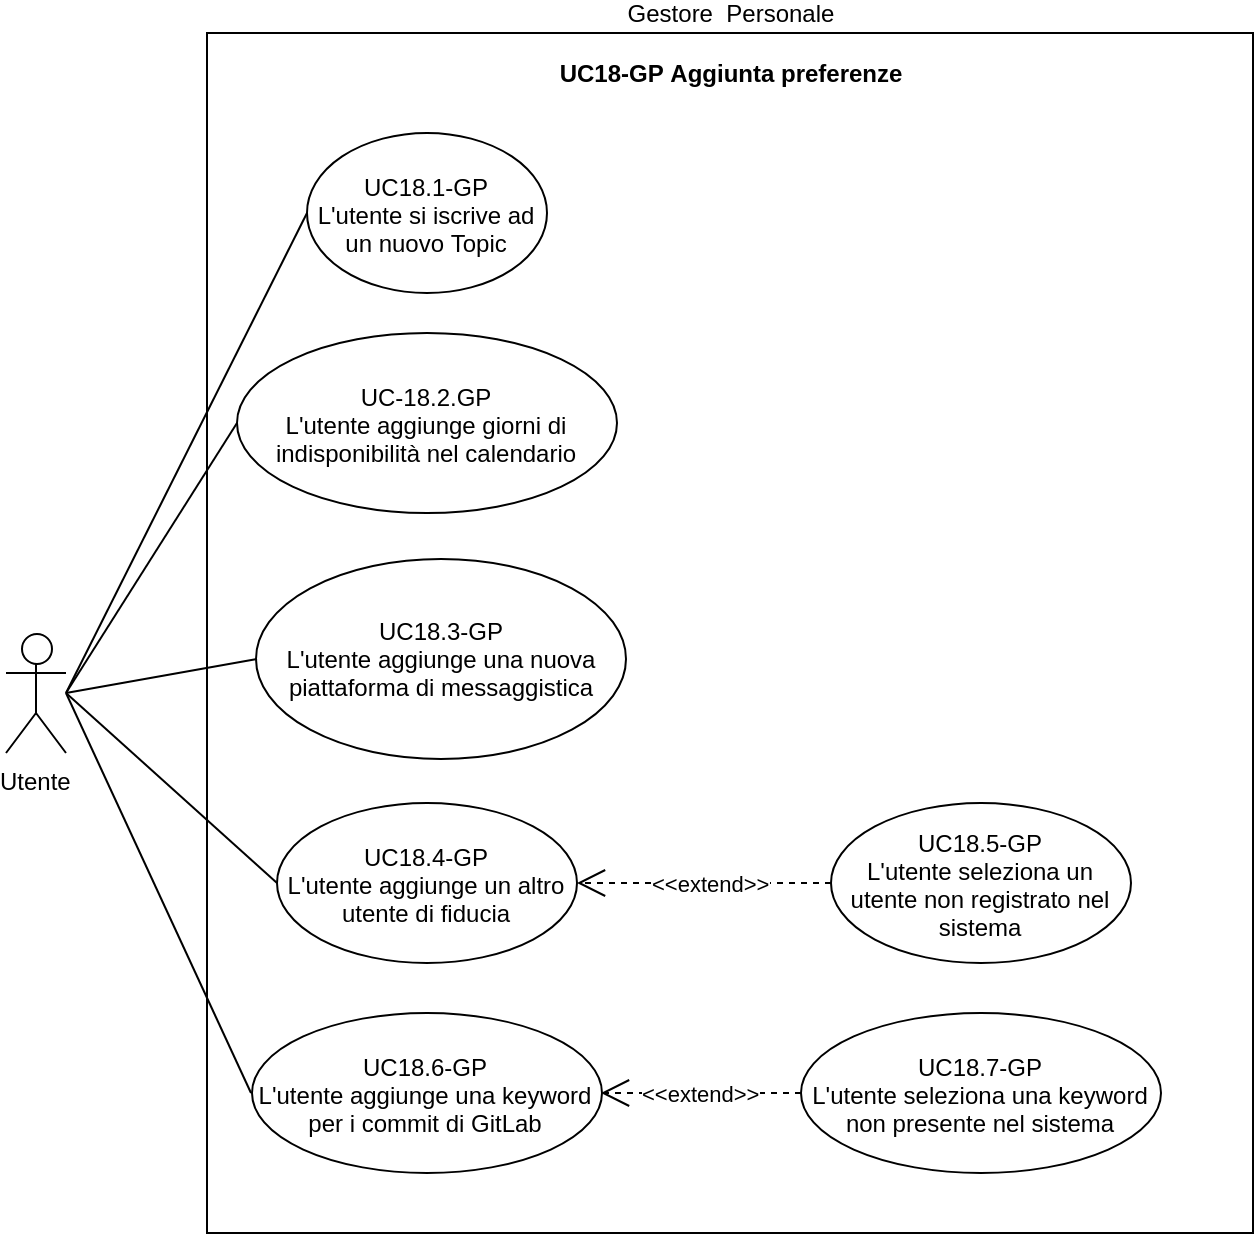
\includegraphics[width=\textwidth]{img/casi_d'uso/UC18.png}\\
			\caption{UC\theuccount-GP - Rimozione preferenze}
		\end{figure}
	\begin{itemize}
		\item \textbf{Codice}: UC\theuccount-GP.
		\item \textbf{Titolo}: rimozione preferenze.
		\item \textbf{Attori primari}: utente.
		\item \textbf{Descrizione}: l’utente, dopo aver selezionato delle preferenze dalle opzioni di configurazione, ne rimuove una o più. Le preferenze consistono in Topic, date di calendario e la piattaforma di messaggistica (Telegram e email).
		\item \textbf{Precondizione}: l’utente ha eseguito l'accesso nel sistema ed è presente almeno	una preferenza selezionata tra quelle proposte da Butterfly.
		\item \textbf{Postcondizione}: la nuova configurazione contiene una o più preferenze in meno rispetto	a quella precedente.
		\item \textbf{Scenario principale}:
		\begin{enumerate}
			\item L'utente procede alla rimozione di una o più preferenze
		\end{enumerate}
	\end{itemize}

	\stepcounter{subuccount}
	\subsubsection{UC\theuccount.\thesubuccount-GP - Disiscrizione Topic}

		\begin{itemize}
			\item \textbf{Codice}: UC\theuccount.\thesubuccount-GP.
			\item \textbf{Titolo}: disiscrizione Topic.
			\item \textbf{Attori primari}: utente.
			\item \textbf{Descrizione}: l’utente si disiscrive da uno o più Topic dai quali prima riceveva delle notifiche.
			\item \textbf{Precondizione}: l’utente ha acceduto correttamente nel sistema e non ha già selezionato tutti i Topic possibili proposti da \progetto.
			\item \textbf{Postcondizione}: il numero di Topic a cui è iscritto l’utente è diminuito.
			\item \textbf{Scenario principale}:
			\begin{enumerate}
				\item L'utente procede alla disiscrizione di uno o più Topic
			\end{enumerate}
		\end{itemize}

	\stepcounter{subuccount}
	\subsubsection{UC\theuccount.\thesubuccount-GP - Rimozione di uno o più giorni di irreperibilità nel calendario}

	\begin{itemize}
		\item \textbf{Codice}: UC\theuccount.\thesubuccount-GP.
		\item \textbf{Titolo}: rimozione di uno o più giorni di irreperibilità nel calendario.
		\item \textbf{Attori primari}: utente.
		\item \textbf{Descrizione}: l’utente rimuove i giorni di calendario in cui precedentemente	non era reperibile, tornando disponibile.
		\item \textbf{Precondizione}: l’utente ha acceduto correttamente nel sistema ed è presente almeno un giorno di calendario selezionato.
		\item \textbf{Postcondizione}: il numero di giorni di calendario in cui l’utente non è reperibile è diminuito.
		\item \textbf{Scenario principale}:
		\begin{enumerate}
			\item L'utente procede alla rimozione di uno o più giorni di irreperibilità
		\end{enumerate}
	\end{itemize}

	\stepcounter{subuccount}
	\subsubsection{UC\theuccount.\thesubuccount-GP - Rimozione preferenza piattaforma di messaggistica}

	\begin{itemize}
		\item \textbf{Codice}: UC\theuccount.\thesubuccount-GP.
		\item \textbf{Titolo}: rimozione preferenza piattaforma di messaggistica.
		\item \textbf{Attori primari}: utente.
		\item \textbf{Descrizione}: l’utente rimuove una o più preferenze tra Telegram e Email dalle	quali non vuole più ricevere notifiche tramite \progetto.
		\item \textbf{Precondizione}: l’utente ha acceduto correttamente nel sistema ed è presente almeno una piattaforma di messaggistica selezionata tra quelle proposte da \progetto.
		\item \textbf{Postcondizione}: il numero di piattaforme di messaggistica da cui l’utente vuole ricevere notifiche è diminuito.
		\item \textbf{Scenario principale}:
		\begin{enumerate}
			\item L'utente procede alla rimozione di una o più piattaforme di messaggistica
		\end{enumerate}
	\end{itemize}

	% \stepcounter{subuccount}
	% \subsubsection{UC\theuccount.\thesubuccount-GP - Rimozione persona di fiducia}

	% \begin{itemize}
	% 	\item \textbf{Codice}: UC\theuccount.\thesubuccount-GP.
	% 	\item \textbf{Titolo}: aggiunta persona di fiducia.
	% 	\item \textbf{Attori primari}: utente.
	% 	\item \textbf{Descrizione}:  l’utente rimuove l'utente legato a un identificativo di sua preferenza a cui inoltrare i messaggi in caso di indisponibilità.
	% 	\item \textbf{Precondizione}: l’utente ha eseguito l'accesso nel sistema e vuole rimuovere la sua persona di fiducia.
	% 	\item \textbf{Postcondizione}: la preferenza viene rimossa correttamente.
	% 	\item \textbf{Scenario principale}:
	% 	\begin{enumerate}
	% 		\item L’utente procede alla rimozione della sua persona di fiducia
	% 	\end{enumerate}
	% 	\item \textbf{Estensioni}:
	% 	\begin{enumerate}
	% 		\item Errore identificativo persona di fiducia inesistente [UC\theuccount.5-GP].
	% 	\end{enumerate}
	% \end{itemize}

	% \stepcounter{subuccount}
	% \subsubsection{UC\theuccount.\thesubuccount-GP - Errore identificativo persona di fiducia inesistente}

	% \begin{itemize}
	% 	\item \textbf{Codice}: UC\theuccount.\thesubuccount-GP.
	% 	\item \textbf{Titolo}: errore identificativo persona di fiducia inesistente.
	% 	\item \textbf{Attori primari}: utente.
	% 	\item \textbf{Descrizione}: l’utente viene avvisato che ha inserito un identificativo errato.
	% 	\item \textbf{Precondizione}: l’utente ha acceduto con le sue credenziali corrette nel sistema e vuole rimuovere la sua persona di fiducia.
	% 	\item \textbf{Postcondizione}: il sistema comunica all’utilizzatore l’errore.
	% 	\item \textbf{Scenario principale}:
	% 	\begin{enumerate}
	% 		\item L'utente inserisce l'identificativo della sua persona di fiducia
	% 		\item Il sistema rileva che questo identificativo non esiste
	% 		\item L'utente visualizza il messaggio di errore
	% 	\end{enumerate}
	% \end{itemize}

	\stepcounter{subuccount}
	\subsubsection{UC\theuccount.\thesubuccount-GP - Rimozione di keyword per i push di GitLab}

	\begin{itemize}
		\item \textbf{Codice}: UC\theuccount.\thesubuccount-GP.
		\item \textbf{Titolo}: rimozione di keyword per i push di GitLab.
		\item \textbf{Attori primari}: utente.
		\item \textbf{Descrizione}: l’utente seleziona e rimuove una o più keyword già presente nel sistema per non ricevere la notifica di push in
		cui i messaggi di commit contengono la keyword rimossa.
		\item \textbf{Precondizione}:  l’utente ha acceduto al sistema.
		\item \textbf{Postcondizione}: nelle nuove configurazioni dell'utente selezionato sono state rimosse delle keyword precedentemente presenti.
		\item \textbf{Scenario principale}:
		\begin{enumerate}
			\item L'utente rimuove una o più keyword per cui non vuole iù ricevere messaggi di push
		\end{enumerate}
		\item \textbf{Estensioni}:
		\begin{enumerate}
			\item Errore keyword da rimuovere non presente [UC\theuccount.7-GP]
		\end{enumerate}
	\end{itemize}

	\stepcounter{subuccount}
	\subsubsection{UC\theuccount.\thesubuccount-GP - Errore keyword da rimuovere non presente}

	\begin{itemize}
		\item \textbf{Codice}: UC\theuccount.\thesubuccount-GP.
		\item \textbf{Titolo}: errore keyword da rimuovere non presente.
		\item \textbf{Attori primari}: utente.
		\item \textbf{Descrizione}: la keyword che l'utente intende rimuovere non è registrata nel sistema.
		\item \textbf{Precondizione}: l’utente ha acceduto al sistema.
		\item \textbf{Postcondizione}: viene visualizzato un messaggio d'errore con indicato che la keyword	selezionata che non è presente nel sistema.
		\item \textbf{Scenario principale}:
		\begin{enumerate}
			\item L'utente inserisce la keyword che vuole rimuovere
			\item Il sistema rileva che non è presente
			\item L'utente visualizza il messaggio di errore
		\end{enumerate}
	\end{itemize}
